% Provenance (never printed): cycle 4 SVT, "La planete Terre": earthquakes,
% faults, seismic waves and their recording, magnitude and intensity, the
% link with plate boundaries; natural hazards (tsunamis) and prevention; see
% sources/book1/PROVENANCE.md. Book 1, grade 7, chapter 3.
% Vocabulary guard: P and S waves are named in prose only (they were named in
% g6.4, defined in Book 2 g11); "sediment" not before g7.4; "intensity" is
% always the earthquake's (homograph with physics: linker STOP list).
\chapter{Earthquakes}\label{ch:g7:earthquakes}

On the morning of 26~December 2004, under the \omterm{def:g2:water-on-earth:ocean}{sea} off the north-western tip
of Sumatra, in Indonesia, the \omterm{def:g3:stones-pebbles-sand:rock}{rocks} broke along a \omterm{def:g7:earthquakes:fault}{fault}: it was one of the
largest \omterm{def:g4:volcanoes-earthquakes-first-look:earthquake}{earthquakes} ever measured. On the nearby \omterm{def:g1:landscapes-around-us:water}{coast} of Sumatra, the
\omterm{def:g2:water-on-earth:ocean}{sea} rose in waves up to \qty{51}{m} high, which swept as far as \qty{5}{km}
inland. Over the next hours the waves crossed the Indian \omterm{def:g2:water-on-earth:ocean}{Ocean} and struck
the \omterm{def:g1:landscapes-around-us:water}{coasts} of fifteen countries, as far away as Africa. About 230\,000
people died. There was, at the time, no warning system in the Indian
\omterm{def:g2:water-on-earth:ocean}{Ocean}.
% ledger: usgs:largest, nws:tsunami-2004

\begin{omfigure}
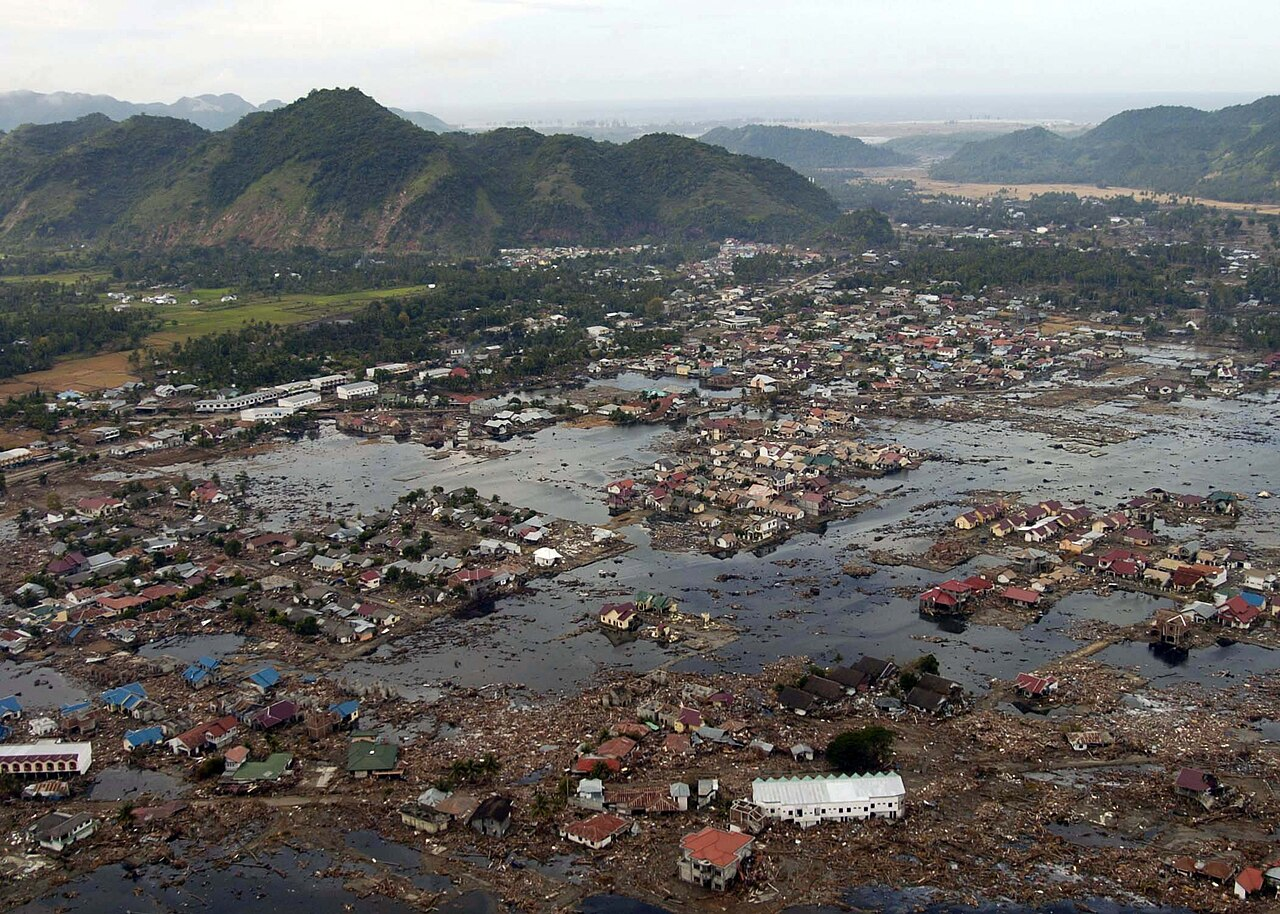
\includegraphics[width=0.78\linewidth]{images/book1/g7-tsunami-village.jpg}

{\small A village near the \omterm{def:g1:landscapes-around-us:water}{coast} of Sumatra a week after the \omterm{def:g7:earthquakes:tsunami}{tsunami} of
26~December 2004. U.S. Navy photograph by Philip~A. McDaniel (public
domain, via Wikimedia Commons).}
% ledger: commons:tsunami-village
\label{fig:g7:earthquakes:tsunami-village}
\end{omfigure}

How do \omterm{def:g3:stones-pebbles-sand:rock}{rocks} break? How do scientists find, within minutes, where an
\omterm{def:g4:volcanoes-earthquakes-first-look:earthquake}{earthquake} struck and how large it was? And why did the \omterm{def:g2:water-on-earth:ocean}{sea}, hours later,
rise on \omterm{def:g1:landscapes-around-us:water}{coasts} where nobody had felt anything?

\begin{recall}
An \emph{\omterm{def:g4:volcanoes-earthquakes-first-look:earthquake}{earthquake}} is a sudden shaking of the ground, caused by \omterm{def:g3:stones-pebbles-sand:rock}{rocks}
that break and slip, deep underground
(\cref{ch:g4:volcanoes-earthquakes-first-look}). The outer shell of the
Earth is made of \omterm{def:g7:plate-tectonics:plate}{plates}, and 92~\% of the large \omterm{def:g4:volcanoes-earthquakes-first-look:earthquake}{earthquakes} happen less
than \qty{300}{km} from a \omterm{def:g7:plate-tectonics:plate-boundary}{plate boundary} (\cref{ch:g7:plate-tectonics}).
When an \omterm{def:g4:volcanoes-earthquakes-first-look:earthquake}{earthquake} strikes, waves travel through the \omterm{def:g3:stones-pebbles-sand:rock}{rocks} of the whole
Earth: a faster kind (the P~waves) and a slower kind (the S~waves); by
timing them, scientists discovered the \omterm{def:g6:inside-the-earth:layers}{core}
(\cref{ch:g6:inside-the-earth}).
\end{recall}

\section{Rocks that break}

The \omterm{def:g7:plate-tectonics:plate}{plates} move a few centimetres a year, but their edges are rough: they
stick together while the rest of the \omterm{def:g7:plate-tectonics:plate}{plates} keeps moving. The \omterm{def:g3:stones-pebbles-sand:rock}{rocks} near
the edge bend a little, like a ruler you push at both ends, and store up
energy. When the push finally overcomes the friction, the \omterm{def:g3:stones-pebbles-sand:rock}{rocks} unstick
all at once and slip: that sudden slip is the \omterm{def:g4:volcanoes-earthquakes-first-look:earthquake}{earthquake}.
% ledger: usgs:eq-basics

\begin{definition}[Fault]\label{def:g7:earthquakes:fault}
A \emph{fault}\index{fault} is a break in the \omterm{def:g3:stones-pebbles-sand:rock}{rocks} along which the two
blocks on either side have moved with respect to each other. During an
\omterm{def:g4:volcanoes-earthquakes-first-look:earthquake}{earthquake} the blocks slip suddenly along the fault; the larger the
fault and the slip, the larger the \omterm{def:g4:volcanoes-earthquakes-first-look:earthquake}{earthquake}.
\end{definition}

A \omterm{def:g7:plate-tectonics:plate-boundary}{plate boundary} is made of many \omterm{def:g7:earthquakes:fault}{faults}, and most of the world's
\omterm{def:g4:volcanoes-earthquakes-first-look:earthquake}{earthquakes} happen on them. But \omterm{def:g7:earthquakes:fault}{faults} also exist inside the \omterm{def:g7:plate-tectonics:plate}{plates}, and
some of them can break too. When a large \omterm{def:g7:earthquakes:fault}{fault} breaks near the surface,
the slip can be seen on the ground: a step in a field, a road cut in two,
a fence or a row of trees shifted sideways.
% ledger: usgs:eq-basics

\begin{omfigure}
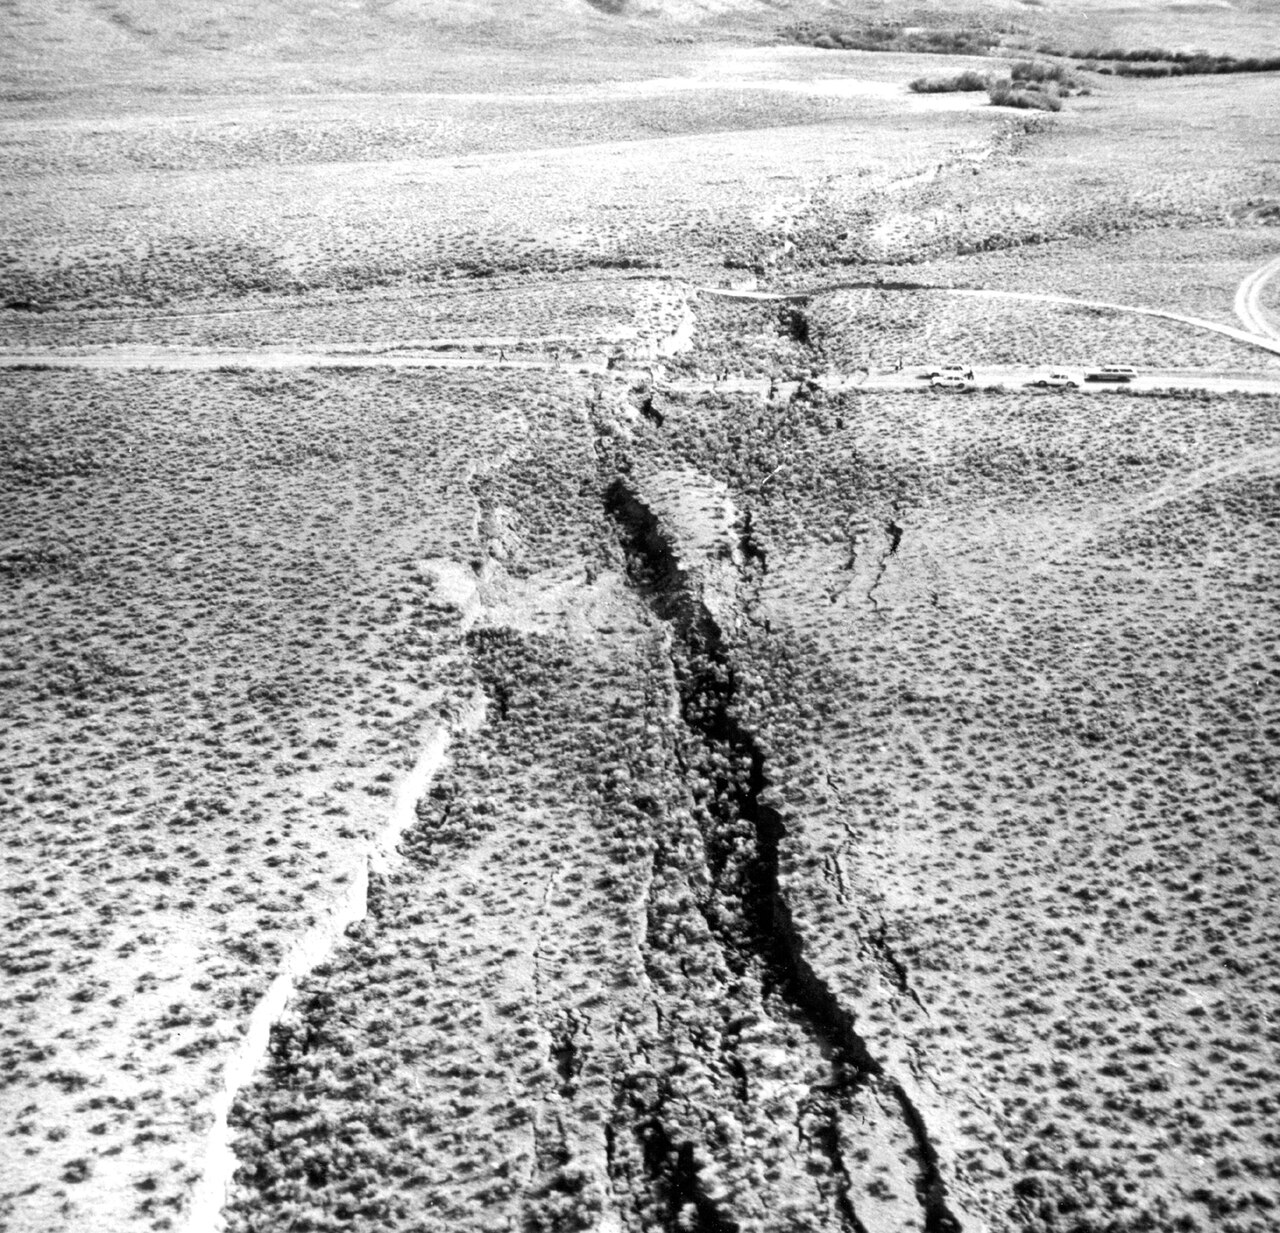
\includegraphics[width=0.62\linewidth]{images/book1/g7-borah-scarp.jpg}

{\small Steps in the ground left by the 1983 Borah Peak \omterm{def:g4:volcanoes-earthquakes-first-look:earthquake}{earthquake}, in
Idaho (United States), seen from the air: along the \omterm{def:g7:earthquakes:fault}{fault}, one side
dropped down with respect to the other, and the step crosses the road at
the top. Photograph: R.~E. Wallace, U.S. Geological Survey (public domain,
via Wikimedia Commons).}
% ledger: commons:borah-scarp
\label{fig:g7:earthquakes:borah}
\end{omfigure}

\begin{definition}[Focus and epicentre]\label{def:g7:earthquakes:focus}
The \emph{focus}\index{focus} of an \omterm{def:g4:volcanoes-earthquakes-first-look:earthquake}{earthquake} is the place underground,
on the \omterm{def:g7:earthquakes:fault}{fault}, where the slip starts. The \emph{epicentre}\index{epicentre}
is the point on the Earth's surface directly above the focus.
\end{definition}

The \omterm{def:g7:earthquakes:focus}{focus} is often a few kilometres to a few tens of kilometres deep. Of
the 7\,031 \omterm{def:g4:volcanoes-earthquakes-first-look:earthquake}{earthquakes} of \omterm{def:g7:earthquakes:magnitude}{magnitude}~6 or more recorded between 1976 and
2025, 5\,561 --- 79~\% --- had their \omterm{def:g7:earthquakes:focus}{focus} less than \qty{70}{km} down.
But 483 started more than \qty{300}{km} down, and the deepest
\qty{688}{km} down: these deep \omterm{def:g4:volcanoes-earthquakes-first-look:earthquake}{earthquakes} happen where one \omterm{def:g7:plate-tectonics:plate}{plate} sinks
under another, inside the sinking \omterm{def:g7:plate-tectonics:plate}{plate}.
% ledger: data:usgs-comcat (figdata/grade-7/quake_counts.py, part depth)

A large \omterm{def:g4:volcanoes-earthquakes-first-look:earthquake}{earthquake} rarely comes alone. It is often followed by smaller ones
in the same place, the \emph{aftershocks}, for weeks, months and even
years. Sometimes smaller \omterm{def:g4:volcanoes-earthquakes-first-look:earthquake}{earthquakes} come before it, but nobody can tell
they were warnings until the large one has happened: scientists cannot
predict \omterm{def:g4:volcanoes-earthquakes-first-look:earthquake}{earthquakes}. They can only say which \omterm{def:g7:earthquakes:fault}{faults} will break again one
day, and help people prepare.
% ledger: usgs:eq-basics, usgs:seismograph

\begin{omfigure}
\begin{tikzpicture}[font=\small, x=1cm, y=1cm]
  % a block of crust seen in perspective: front face and top face
  \def\dx{2.2}\def\dy{1.3}
  % top surface: two blocks separated by the fault trace
  \fill[green!12] (0,0) -- (4.6,0) -- (4.6+\dx,\dy) -- (\dx,\dy) -- cycle;
  \fill[green!18] (4.6,0) -- (9,0) -- (9+\dx,\dy) -- (4.6+\dx,\dy) -- cycle;
  % front face
  \fill[brown!30] (0,0) -- (4.6,0) -- (3.4,-4) -- (0,-4) -- cycle;
  \fill[brown!40] (4.6,0) -- (9,0) -- (9,-4) -- (3.4,-4) -- cycle;
  % right face
  \fill[brown!22] (9,0) -- (9+\dx,\dy) -- (9+\dx,\dy-4) -- (9,-4) -- cycle;
  % fault plane on the front face and trace on top
  \draw[very thick, red!70!black] (4.6,0) -- (3.4,-4);
  \draw[very thick, red!70!black] (4.6,0) -- (4.6+\dx,\dy);
  % slip arrows
  \draw[-{Stealth[length=2.5mm]}, thick] (2.6,-0.35) -- (1.6,-0.35);
  \draw[-{Stealth[length=2.5mm]}, thick] (6.4,-0.35) -- (7.4,-0.35);
  \node[font=\footnotesize, anchor=south] at (2.1,-0.3) {block 1};
  \node[font=\footnotesize, anchor=south] at (6.9,-0.3) {block 2};
  % focus and waves
  \coordinate (F) at (3.95,-2.4);
  \foreach \r in {0.5,1.0,1.5,2.0}
    \draw[blue!60, dashed] (F) circle (\r);
  \fill[red!80!black] (F) circle (0.13);
  % epicentre: on the surface, straight above the focus (front edge of the top face)
  \coordinate (E) at (3.95,0);
  \draw[black!60, densely dotted, thick] (F) -- (E);
  \node[star, star points=5, star point ratio=2.4, fill=orange, draw=black, inner sep=1.4pt] at (E) {};
  % labels
  \node[anchor=west] at (9.5,-2.3) {focus};
  \draw[black!60] (9.45,-2.3) -- (4.1,-2.4);
  \node[anchor=south west] at (4.9,1.9) {epicentre};
  \draw[black!60] (4.95,1.95) -- (4.05,0.12);
  \node[anchor=south, red!70!black] at (6.8,1.3) {fault};
  \node[anchor=east, blue!60!black, align=right] at (-0.15,-2.6) {waves spread\\in all directions};
  \draw[blue!60, -{Stealth}] (-0.1,-2.6) -- (1.9,-2.5);
\end{tikzpicture}

{\small A \omterm{def:g7:earthquakes:fault}{fault}, the \omterm{def:g7:earthquakes:focus}{focus} and the \omterm{def:g7:earthquakes:focus}{epicentre} (a drawing, not to scale).
The two blocks slip past each other along the \omterm{def:g7:earthquakes:fault}{fault} (red); the slip starts
at the \omterm{def:g7:earthquakes:focus}{focus}, and waves spread out from it in all directions, like ripples
on a pond. The \omterm{def:g7:earthquakes:focus}{epicentre} (star) is on the surface, straight above the
\omterm{def:g7:earthquakes:focus}{focus}.}
% ledger: usgs:eq-basics
\label{fig:g7:earthquakes:fault}
\end{omfigure}


\section{Recording an earthquake}

\begin{definition}[Seismometer and seismogram]\label{def:g7:earthquakes:seismometer}
A \emph{seismometer}\index{seismometer} is an instrument that records the
shaking of the ground. Its record, a wiggly line drawn against time, is a
\emph{seismogram}\index{seismogram}.
\end{definition}

The idea of a \omterm{def:g7:earthquakes:seismometer}{seismometer} is simple. A frame is fixed firmly to the
ground; a heavy weight hangs from it on a spring. When the ground shakes,
the frame shakes with it, but the heavy weight, held only by its spring,
stays almost still. The instrument records the movement of the frame with
respect to the still weight: that is the movement of the ground. In the
drawing below, a pen fixed to the mass draws it on paper wrapped around a
turning drum.
% ledger: usgs:seismograph

\begin{omfigure}
\begin{tikzpicture}[font=\small, x=1cm, y=1cm]
  \begin{scope}
    % ground
    \fill[brown!30] (-0.6,-0.6) rectangle (5.0,0);
    \draw[decorate, decoration={snake, amplitude=1.2pt, segment length=6pt}, brown!70!black, thick]
      (-0.6,0) -- (5.0,0);
    % frame
    \fill[black!55] (0,0) rectangle (0.25,3.2);
    \fill[black!55] (0,3.0) rectangle (2.4,3.25);
    % spring and weight
    \draw[decorate, decoration={coil, aspect=0.5, segment length=3pt, amplitude=4pt}, thick]
      (2.1,3.0) -- (2.1,2.1);
    \fill[black!80] (1.7,1.45) rectangle (2.5,2.1);
    \node[white, font=\scriptsize] at (2.1,1.78) {mass};
    % pen arm and drum
    \draw[thick] (2.5,1.75) -- (3.45,1.75);
    \fill (3.45,1.75) circle (0.05);
    \draw[thick, fill=white] (3.95,1.75) circle (0.5);
    \draw[thick] (3.95,1.25) -- (3.95,0);
    \draw[-{Stealth}, black!60] (4.55,2.2) arc (40:-40:0.7);
    % labels
    \node[anchor=east, align=right, font=\footnotesize] at (-0.1,2.3) {frame fixed\\to the ground};
    \node[anchor=west, font=\footnotesize] at (2.6,2.65) {spring};
    \draw[black!60] (2.55,2.65) -- (2.25,2.6);
    \node[anchor=north, align=center, font=\footnotesize] at (2.1,1.35) {heavy mass:\\stays still};
    \node[anchor=west, align=left, font=\footnotesize] at (4.7,1.05) {turning drum\\with paper};
    \node[anchor=north, font=\footnotesize] at (2.2,-0.65) {the ground shakes};
  \end{scope}
  \begin{scope}[xshift=7.2cm, yshift=0.4cm]
    \begin{axis}[width=7.6cm, height=4.2cm, xmin=0, xmax=60, ymin=-1.1, ymax=1.1,
        axis x line=bottom, axis y line=none, xlabel={time (seconds)},
        tick label style={font=\scriptsize}, label style={font=\footnotesize}, clip=false]
      \addplot[black, line width=0.4pt] table[x=t, y=v] {figdata/out/grade-7-epicentre-m-trace.dat};
      \draw[blue!70!black, -{Stealth[length=2mm]}] (axis cs:10,1.45) -- (axis cs:10,0.45);
      \node[blue!70!black, font=\scriptsize, anchor=south east] at (axis cs:10.5,1.45) {faster waves arrive};
      \draw[red!70!black, -{Stealth[length=2mm]}] (axis cs:20,1.45) -- (axis cs:20,1.05);
      \node[red!70!black, font=\scriptsize, anchor=south west] at (axis cs:19.5,1.45) {slower waves arrive};
      \draw[{Stealth[length=2mm]}-{Stealth[length=2mm]}] (axis cs:10,-0.75) -- (axis cs:20,-0.75);
      \node[font=\scriptsize, anchor=east] at (axis cs:9,-0.75) {delay: 10 s};
    \end{axis}
  \end{scope}
\end{tikzpicture}

{\small Left: the principle of a \omterm{def:g7:earthquakes:seismometer}{seismometer} (a drawing). Right: a
\omterm{def:g7:earthquakes:seismometer}{seismogram} drawn for this book (not a real record): the line is calm,
then the faster waves arrive, then, ten seconds later, the slower and
larger ones.}
% ledger: usgs:seismograph (trace drawn by figdata/grade-7/epicentre.py, part m-trace)
\label{fig:g7:earthquakes:seismometer}
\end{omfigure}

\subsection*{How far away was the earthquake?}

A \omterm{def:g7:earthquakes:seismometer}{seismogram} tells more than ``the ground shook''. The faster waves always
arrive first and the slower ones after. Close to the \omterm{def:g7:earthquakes:focus}{focus}, they arrive
almost together; far away, the slower waves fall more and more behind,
just as during a \omterm{def:g5:natural-hazards:storm}{storm} the thunder lags farther behind the lightning when
the \omterm{def:g5:natural-hazards:storm}{storm} is far away. So the delay between the two arrivals tells the
distance to the \omterm{def:g4:volcanoes-earthquakes-first-look:earthquake}{earthquake}.
% ledger: usgs:seismograph

How many kilometres for each second of delay? It depends on the speeds of
the two waves in the \omterm{def:g3:stones-pebbles-sand:rock}{rocks} they cross. With the speeds of the reference
model of the Earth (\cref{ch:g6:inside-the-earth}), each second of delay
means about \qty{7}{km} in the upper \omterm{def:g6:inside-the-earth:layers}{crust} and \qty{9}{km} in the lower
\omterm{def:g6:inside-the-earth:layers}{crust}. In the exercises of this chapter we use the round value of
\qty{8}{km} for each second.
% ledger: data:prem (computed in figdata/grade-7/epicentre.py, part rule)

\begin{method}[Finding the epicentre with three stations]\label{met:g7:earthquakes:three-circles}
\begin{enumerate}
  \item On the \omterm{def:g7:earthquakes:seismometer}{seismogram} of each station, read the delay between the
        arrival of the faster waves and the arrival of the slower ones.
  \item Turn each delay into a distance (here: $8 \times$ the delay in
        seconds, in kilometres).
  \item On a \omterm{def:g2:drawing-to-map:map}{map}, draw around each station a circle whose radius is its
        distance. The \omterm{def:g7:earthquakes:focus}{epicentre} lies somewhere on each circle.
  \item With two circles, there are usually two possible points; the third
        circle passes through only one of them: that is the \omterm{def:g7:earthquakes:focus}{epicentre}.
\end{enumerate}
\end{method}

\begin{example}[Three circles]\label{ex:g7:earthquakes:three-circles}
Three stations record the same \omterm{def:g4:volcanoes-earthquakes-first-look:earthquake}{earthquake}. The delays are \qty{10}{s} at
station~M1, \qty{11.25}{s} at M2 and \qty{9.75}{s} at M3. The distances are
$8 \times 10 = \qty{80}{km}$, $8 \times 11.25 = \qty{90}{km}$ and
$8 \times 9.75 = \qty{78}{km}$. The three circles, drawn below, meet at a
single point: the \omterm{def:g7:earthquakes:focus}{epicentre}.
% ledger: usgs:seismograph (figdata/grade-7/epicentre.py, parts m-stations and m-circles)
\end{example}

\begin{omfigure}
\begin{tikzpicture}
  \begin{axis}[axis equal image, width=8.2cm, xmin=-150, xmax=170, ymin=-160, ymax=160,
      xtick={-120,-80,...,160}, ytick={-120,-80,...,120}, grid=both, grid style={black!12},
      tick label style={font=\scriptsize}, xlabel={km}, ylabel={km}, label style={font=\footnotesize}]
    \addplot[blue!60!black, line width=0.6pt] table[x=x, y=y] {figdata/out/grade-7-epicentre-m-circles.dat};
    \addplot[only marks, mark=triangle*, mark size=3pt, black,
        nodes near coords, point meta=explicit symbolic,
        nodes near coords style={font=\scriptsize, anchor=north, yshift=-2pt}]
      table[x=x, y=y, meta=name] {figdata/out/grade-7-epicentre-m-stations.dat};
    \node[star, star points=5, star point ratio=2.4, fill=orange, draw=black, inner sep=1.6pt] at (axis cs:0,0) {};
    \draw[black!60] (axis cs:-4,-4) -- (axis cs:-60,-75);
    \node[font=\scriptsize, anchor=north east, inner sep=1pt] at (axis cs:-60,-75) {epicentre};
  \end{axis}
\end{tikzpicture}

{\small Each circle is centred on a station (triangle), with a radius equal
to that station's distance from the \omterm{def:g4:volcanoes-earthquakes-first-look:earthquake}{earthquake}. The three circles meet at
only one point, the \omterm{def:g7:earthquakes:focus}{epicentre} (star).}
% ledger: usgs:seismograph (figdata/grade-7/epicentre.py, parts m-stations and m-circles)
\label{fig:g7:earthquakes:three-circles}
\end{omfigure}

\begin{omfigure}
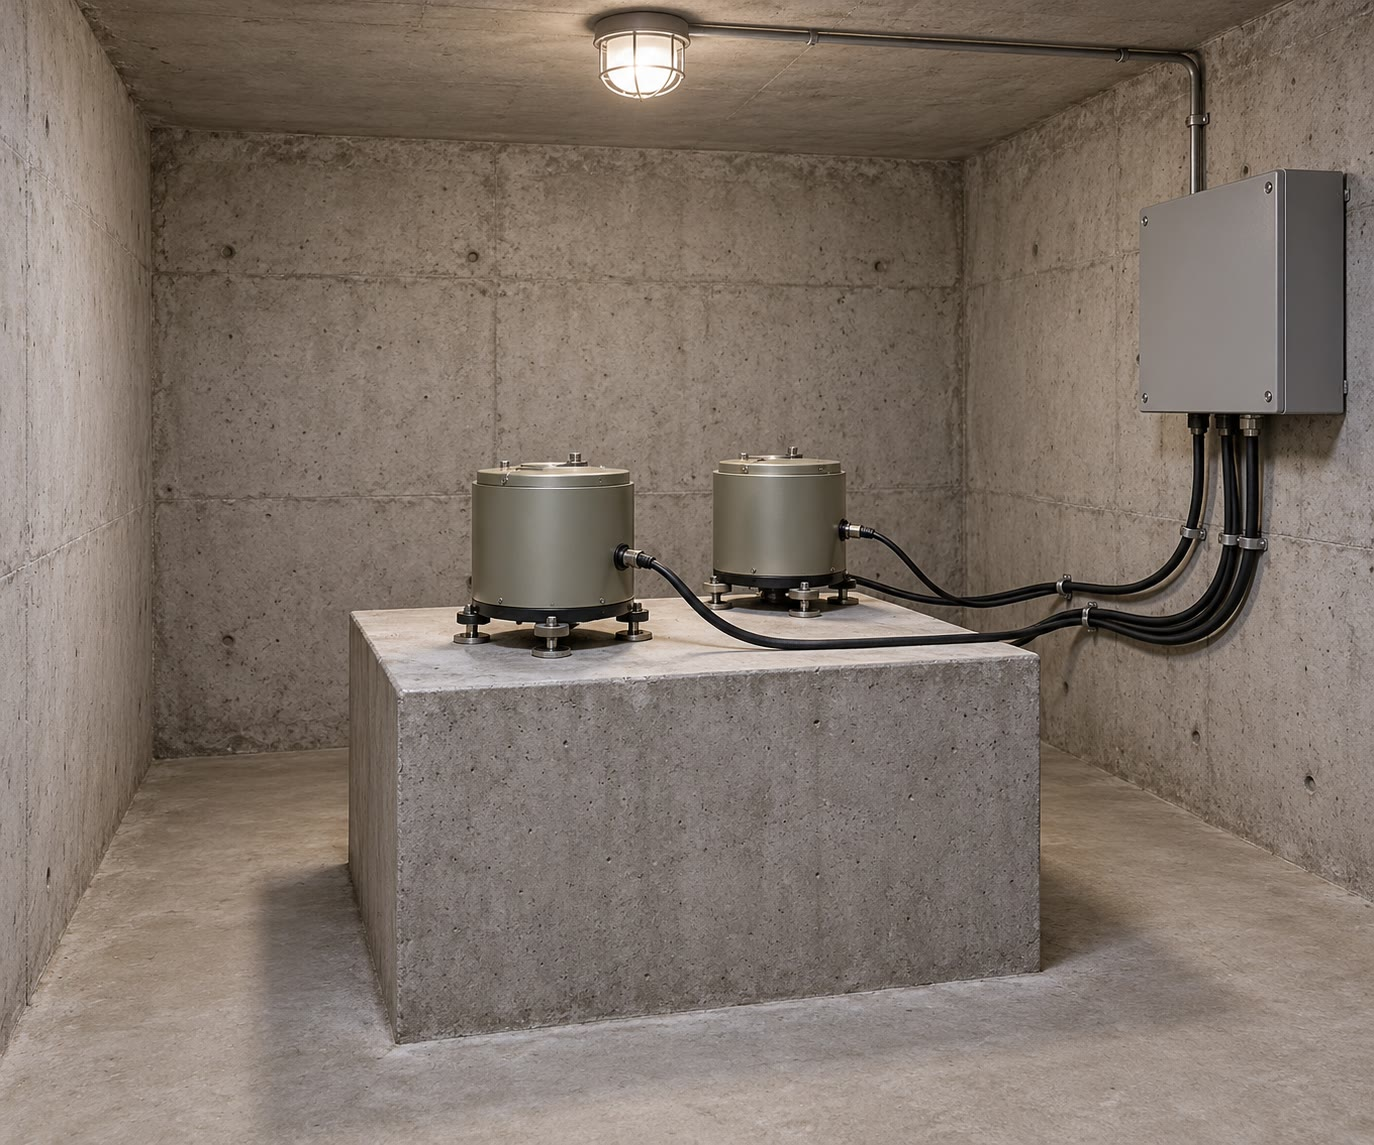
\includegraphics[width=0.58\linewidth]{images/book1/ai/g7-seismometer-vault.jpg}

{\small \omterm{def:g7:earthquakes:seismometer}{Seismometers} in a quiet underground room, set on a concrete pier
that rests on the \omterm{def:g3:stones-pebbles-sand:rock}{rock}, far from roads and machines (AI-generated
illustration of a generic scene).}
\label{fig:g7:earthquakes:vault}
\end{omfigure}

\section{How large? Magnitude and intensity}

Two different numbers describe an \omterm{def:g4:volcanoes-earthquakes-first-look:earthquake}{earthquake}, and they are often confused.

\begin{definition}[Magnitude]\label{def:g7:earthquakes:magnitude}
The \emph{magnitude}\index{magnitude} of an \omterm{def:g4:volcanoes-earthquakes-first-look:earthquake}{earthquake} measures its size:
the energy released at the source. It is worked out from the \omterm{def:g7:earthquakes:seismometer}{seismograms}.
Each \omterm{def:g4:volcanoes-earthquakes-first-look:earthquake}{earthquake} has a single magnitude, written with one decimal, such as
6.3 or 9.1.
\end{definition}

\begin{definition}[Intensity]\label{def:g7:earthquakes:intensity}
The \emph{intensity}\index{intensity} of an \omterm{def:g4:volcanoes-earthquakes-first-look:earthquake}{earthquake} at a place describes
how strongly the ground shook there, from what people felt and from the
damage they saw. It is written in Roman numerals, from I (not felt) to XII
(total destruction). One \omterm{def:g4:volcanoes-earthquakes-first-look:earthquake}{earthquake} has many intensities: a different one
in each place.
\end{definition}

The magnitude scale climbs fast. Each step of 1 in \omterm{def:g7:earthquakes:magnitude}{magnitude} means
waves about 10~times larger on the \omterm{def:g7:earthquakes:seismometer}{seismogram} and about 32~times more
energy released. An \omterm{def:g4:volcanoes-earthquakes-first-look:earthquake}{earthquake} of \omterm{def:g7:earthquakes:magnitude}{magnitude}~8 releases about
$32 \times 32 \approx 1000$ times more energy than one of \omterm{def:g7:earthquakes:magnitude}{magnitude}~6.
% ledger: usgs:mag-energy

\begin{method}[Comparing two magnitudes]\label{met:g7:earthquakes:magnitudes}
To compare the energy of two \omterm{def:g4:volcanoes-earthquakes-first-look:earthquake}{earthquakes}, count the whole steps between
their \omterm{def:g7:earthquakes:magnitude}{magnitudes}, and multiply by 32 once for each step: 1~step, 32~times;
2~steps, about 1000~times; 3~steps, about 32\,000~times.
\end{method}

\begin{example}[Magnitude 9 and magnitude 7]\label{ex:g7:earthquakes:nine-seven}
The 2004 \omterm{def:g4:volcanoes-earthquakes-first-look:earthquake}{earthquake} off Sumatra had a \omterm{def:g7:earthquakes:magnitude}{magnitude} of 9.1. An \omterm{def:g4:volcanoes-earthquakes-first-look:earthquake}{earthquake} of
\omterm{def:g7:earthquakes:magnitude}{magnitude}~7.1 is two steps smaller: it released about
$32 \times 32 = 1024$, so about 1000~times, less energy.
% ledger: usgs:largest, usgs:mag-energy
\end{example}

The largest \omterm{def:g4:volcanoes-earthquakes-first-look:earthquake}{earthquakes} ever measured all happened where one \omterm{def:g7:plate-tectonics:plate}{plate} sinks
under another: \omterm{def:g7:earthquakes:magnitude}{magnitude}~9.5 in Chile on 22~May 1960, 9.2 in Alaska in
1964, 9.1 off Sumatra in 2004 and 9.1 off the \omterm{def:g1:landscapes-around-us:water}{coast} of Japan on 11~March
2011. Large \omterm{def:g4:volcanoes-earthquakes-first-look:earthquake}{earthquakes} are rare, and the larger they are, the rarer, as
the chart shows: each step up in \omterm{def:g7:earthquakes:magnitude}{magnitude}, about ten times fewer.
% ledger: usgs:largest, data:usgs-comcat

\begin{omfigure}
\begin{tikzpicture}
  \begin{axis}[ybar, width=0.72\linewidth, height=5.4cm, bar width=22pt,
      ymode=log, log origin y=infty, ymin=0.01, ymax=600,
      xtick=data, xticklabels from table={figdata/out/grade-7-quake_counts.dat}{label},
      xlabel={magnitude}, ylabel={earthquakes per year},
      ytick={0.01,0.1,1,10,100}, yticklabels={0.01,0.1,1,10,100},
      tick label style={font=\scriptsize}, label style={font=\small},
      nodes near coords, point meta=explicit symbolic,
      nodes near coords style={font=\scriptsize}, enlarge x limits=0.18,
      axis x line*=bottom, axis y line*=left]
    \addplot[fill=omThm!45, draw=omThm!80!black] table[x=cls, y=per_year, meta=per_year] {figdata/out/grade-7-quake_counts.dat};
  \end{axis}
\end{tikzpicture}

{\small \omterm{def:g4:volcanoes-earthquakes-first-look:earthquake}{Earthquakes} per year, on average over 1976--2025, by \omterm{def:g7:earthquakes:magnitude}{magnitude}.
The vertical scale is special: each line is ten times the one below it.
Data: U.S. Geological Survey \omterm{def:g4:volcanoes-earthquakes-first-look:earthquake}{earthquake} catalogue (7\,031 \omterm{def:g4:volcanoes-earthquakes-first-look:earthquake}{earthquakes} of
\omterm{def:g7:earthquakes:magnitude}{magnitude}~6 or more).}
% ledger: data:usgs-comcat (figdata/grade-7/quake_counts.py, main table)
\label{fig:g7:earthquakes:counts}
\end{omfigure}

The \omterm{def:g7:earthquakes:intensity}{intensity scale} has no formula: it is a list of what happens. The
table gives it in short form.
% ledger: usgs:mmi, usgs:mmi-page

\begin{center}
\small
\begin{tabular}{|c|p{0.8\linewidth}|}
\hline
\textbf{\omterm{def:g7:earthquakes:intensity}{intensity}} & \textbf{what is felt and seen} \\
\hline
I & not felt, except by a very few people \\
II & felt only by a few people at rest, especially upstairs; hanging objects may swing \\
III & felt indoors; it feels like a passing truck \\
IV & felt indoors by many; dishes, windows and doors rattle \\
V & felt by nearly everyone, many woken up; some dishes and windows broken \\
VI & felt by all, many frightened; some heavy furniture moved; slight damage \\
VII & little damage in well-built buildings, much in poorly built ones; some chimneys broken \\
VIII & much damage in ordinary buildings, some partly collapse; chimneys and walls fall \\
IX & great damage even in strong buildings; buildings shifted off their foundations \\
X & most buildings destroyed with their foundations; rails bent \\
XI & few buildings left standing; bridges destroyed \\
XII & damage total; objects thrown into the air \\
\hline
\end{tabular}
\end{center}
% ledger: usgs:mmi

The \omterm{def:g7:earthquakes:intensity}{intensity} is highest, usually, near the \omterm{def:g7:earthquakes:focus}{epicentre}, and decreases with
distance. But it also depends on the ground: solid \omterm{def:g3:stones-pebbles-sand:rock}{rock} shakes the least,
soft \omterm{def:g3:stones-pebbles-sand:sand}{mud} the most. A town built on soft ground can be shaken harder than
another town closer to the \omterm{def:g7:earthquakes:focus}{epicentre} but built on \omterm{def:g3:stones-pebbles-sand:rock}{rock}.
% ledger: usgs:mag-energy

\begin{omfigure}
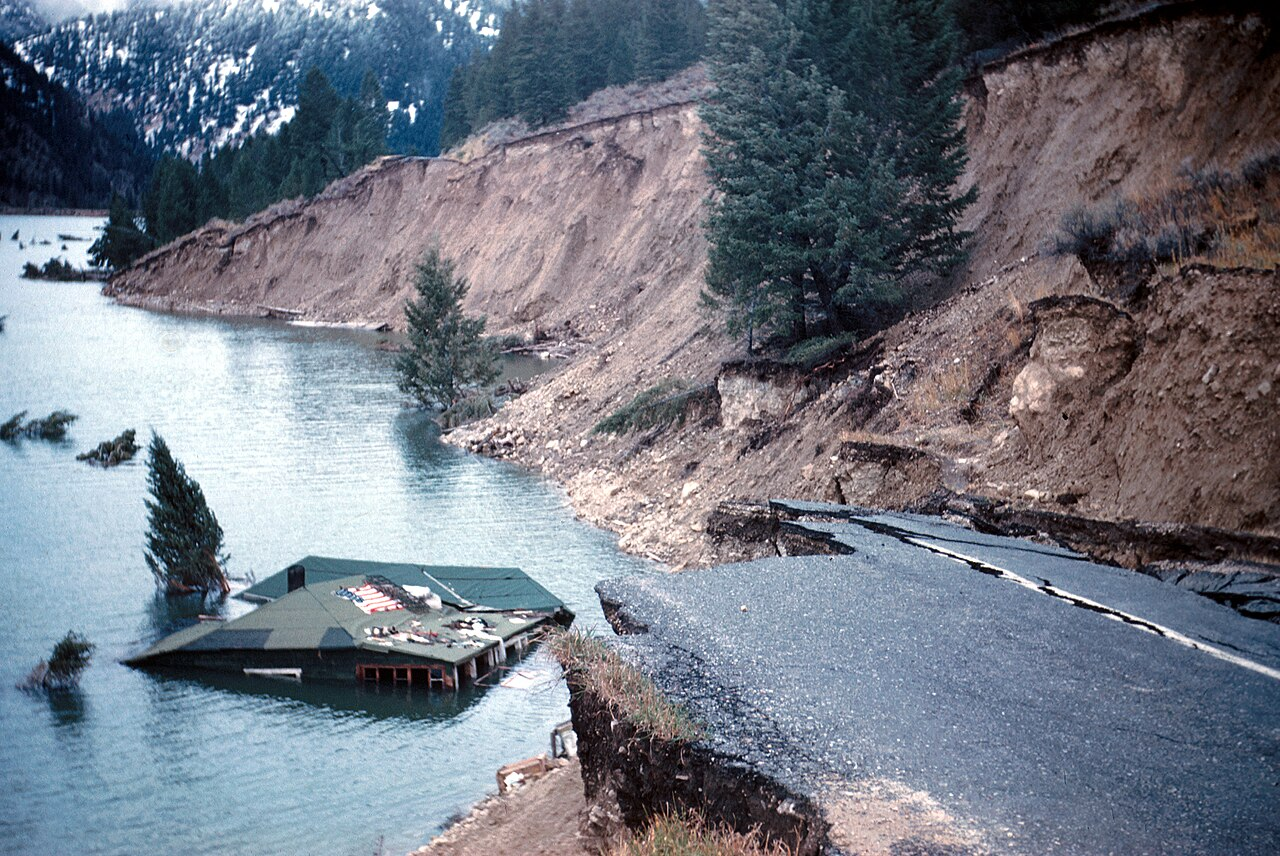
\includegraphics[width=0.6\linewidth]{images/book1/g7-hebgen-road.jpg}

{\small After the Hebgen \omterm{def:g1:landscapes-around-us:water}{Lake} \omterm{def:g4:volcanoes-earthquakes-first-look:earthquake}{earthquake}, Montana (United States), August
1959: the road along the \omterm{def:g1:landscapes-around-us:water}{lake} slumped into the water, and a lodge ended up
almost under water. Damage like this is the mark of a high \omterm{def:g7:earthquakes:intensity}{intensity}.
Photograph: I.~J. Witkind, U.S. Geological Survey (public domain, via
Wikimedia Commons).}
% ledger: commons:hebgen-road, usgs:mmi
\label{fig:g7:earthquakes:hebgen}
\end{omfigure}

\section{Tsunamis}

\begin{definition}[Tsunami]\label{def:g7:earthquakes:tsunami}
A \emph{tsunami}\index{tsunami} is a series of \omterm{def:g2:water-on-earth:ocean}{sea} waves set off by a
sudden movement of the \omterm{def:g2:water-on-earth:ocean}{sea} floor --- usually an \omterm{def:g4:volcanoes-earthquakes-first-look:earthquake}{earthquake} under the \omterm{def:g2:water-on-earth:ocean}{sea},
sometimes an \omterm{def:g4:volcanoes-earthquakes-first-look:eruption}{eruption} --- which can cross whole \omterm{def:g2:water-on-earth:ocean}{oceans} and \omterm{def:g5:water-shapes-the-land:flood}{flood} the
\omterm{def:g1:landscapes-around-us:water}{coasts}.
\end{definition}

When a \omterm{def:g7:earthquakes:fault}{fault} under the \omterm{def:g2:water-on-earth:ocean}{sea} breaks, the \omterm{def:g2:water-on-earth:ocean}{sea} floor moves suddenly up or
down, and lifts or lowers the whole column of water above it. The water spreads out in waves. Out in the deep \omterm{def:g2:water-on-earth:ocean}{ocean}, a \omterm{def:g7:earthquakes:tsunami}{tsunami}
is surprising: it is rarely more than a metre high, and ships do not even
notice it pass beneath them. But it is fast: over \qty{800}{km/h}, as fast
as a jet plane. As it reaches shallow water near the \omterm{def:g1:landscapes-around-us:water}{coast}, it slows down
to 30 or \qty{50}{km/h} --- still faster than anyone can run --- and grows
taller. Most \omterm{def:g7:earthquakes:tsunami}{tsunamis} are less than \qty{3}{m} high at the \omterm{def:g1:landscapes-around-us:water}{coast}; the
largest pass \qty{30}{m}. The first wave is not always the largest, and
the waves can keep coming for hours.
% ledger: nws:tsunami-speed, nws:tsunami-safety

\begin{omfigure}
\begin{tikzpicture}[font=\small, x=1cm, y=1cm]
  % sea floor profile: deep ocean on the left, shelf and coast on the right
  \fill[omSea!35] (0,0) -- (13.2,0) -- (13.2,-0.2) -- (11.4,-0.45) -- (10.2,-1.0) -- (8.8,-2.6) -- (0,-2.6) -- cycle;
  \fill[brown!35] (0,-2.6) -- (8.8,-2.6) -- (10.2,-1.0) -- (11.4,-0.45) -- (13.2,-0.2) -- (13.2,0.5) -- (14.2,1.0) -- (14.2,-3.3) -- (0,-3.3) -- cycle;
  % the broken fault under the sea, at left; one block lifted
  \draw[very thick, red!70!black] (1.9,-3.3) -- (2.3,-2.6);
  \draw[-{Stealth[length=2mm]}, thick] (2.75,-3.1) -- (2.75,-2.75);
  \node[anchor=north west, font=\footnotesize, red!70!black] at (0.1,-3.35) {the fault breaks, the sea floor jumps};
  % wave: low and long in the deep ocean, short and tall near the coast
  \draw[blue!70!black, thick] (0,0) .. controls (1.2,0.18) and (2.2,0.18) .. (3.4,0)
     -- (5.0,0) .. controls (5.8,0.12) and (6.6,0.12) .. (7.4,0) -- (10.6,0)
     .. controls (11.0,0.55) and (11.6,0.9) .. (12.1,0) -- (13.2,0);
  \node[align=center, font=\footnotesize] at (2.0,0.85) {deep ocean: about 1 m high,\\over 800 km/h};
  \node[align=center, font=\footnotesize] at (11.1,1.55) {near the coast: slower\\(30 to 50 km/h), much taller};
  \draw[-{Stealth[length=2.5mm]}, thick, blue!70!black] (4.4,0.45) -- (6.4,0.45);
  \node[font=\footnotesize] at (6.0,-1.5) {thousands of metres deep};
  \node[font=\footnotesize] at (12.0,-0.75) {shallow};
\end{tikzpicture}

{\small A \omterm{def:g7:earthquakes:tsunami}{tsunami} crossing the \omterm{def:g2:water-on-earth:ocean}{ocean} (a drawing, not to scale: the height
of the wave is greatly exaggerated). It is low and very fast over the deep
\omterm{def:g2:water-on-earth:ocean}{ocean}; it slows down and grows in shallow water near the \omterm{def:g1:landscapes-around-us:water}{coast}.}
% ledger: nws:tsunami-speed
\label{fig:g7:earthquakes:tsunami}
\end{omfigure}

\begin{example}[From Sumatra to Sri Lanka]\label{ex:g7:earthquakes:colombo}
Colombo, the largest city of Sri Lanka, is about \qty{1830}{km} from the
\omterm{def:g7:earthquakes:focus}{epicentre} of the 2004 \omterm{def:g4:volcanoes-earthquakes-first-look:earthquake}{earthquake}. At \qty{800}{km/h}, a \omterm{def:g7:earthquakes:tsunami}{tsunami} covers
this distance in $1830 \div 800 \approx 2.3$~hours, that is about 2~hours
and 17~minutes. Nobody in Sri Lanka felt the \omterm{def:g4:volcanoes-earthquakes-first-look:earthquake}{earthquake}: the wave came
without any warning but the \omterm{def:g2:water-on-earth:ocean}{sea} itself.
% ledger: nws:tsunami-speed, usgs:largest (distance and time in figdata/grade-7/quake_counts.py, part tsunami)
\end{example}

\begin{remark}[The warning the sea gives]\label{rem:g7:earthquakes:natural-warning}
% ledger: nws:tsunami-natural-warning, nws:tsunami-speed, shakeout:dch
On a \omterm{def:g1:landscapes-around-us:water}{coast}, three signs can announce a \omterm{def:g7:earthquakes:tsunami}{tsunami}: a strong or long
\omterm{def:g4:volcanoes-earthquakes-first-look:earthquake}{earthquake}; the \omterm{def:g2:water-on-earth:ocean}{sea} behaving strangely --- a sudden \omterm{def:g5:water-shapes-the-land:flood}{flood}, or the water
drawing back far from the shore, showing the \omterm{def:g2:water-on-earth:ocean}{sea} floor like a very low
tide; or a loud roar coming from the \omterm{def:g2:water-on-earth:ocean}{ocean}. During the shaking, protect
yourself as you learned (drop, cover, hold on). Then do not wait for an
official warning: go as high, or as far inland, as you can, at once. A
\omterm{def:g7:earthquakes:tsunami}{tsunami} from a nearby \omterm{def:g4:volcanoes-earthquakes-first-look:earthquake}{earthquake} can arrive within minutes.
\end{remark}


\section{Exercises}

\begin{exercise}[$\star$]\label{exo:g7:earthquakes:1}
Match each word with its meaning: \omterm{def:g7:earthquakes:fault}{fault}; \omterm{def:g7:earthquakes:focus}{focus}; \omterm{def:g7:earthquakes:focus}{epicentre}; \omterm{def:g7:earthquakes:seismometer}{seismometer};
\omterm{def:g7:earthquakes:magnitude}{magnitude}; \omterm{def:g7:earthquakes:intensity}{intensity}. (a) The place underground where the slip starts. (b)
How strongly the ground shook at one place. (c) A break in the \omterm{def:g3:stones-pebbles-sand:rock}{rocks} along
which the two sides have moved. (d) The point on the surface above the
\omterm{def:g7:earthquakes:focus}{focus}. (e) The size of an \omterm{def:g4:volcanoes-earthquakes-first-look:earthquake}{earthquake}, one number for each \omterm{def:g4:volcanoes-earthquakes-first-look:earthquake}{earthquake}. (f)
An instrument that records the shaking of the ground.
\end{exercise}

\begin{exercise}[$\star$]\label{exo:g7:earthquakes:2}
The \omterm{def:g7:earthquakes:focus}{focus} of an \omterm{def:g4:volcanoes-earthquakes-first-look:earthquake}{earthquake} lies \qty{30}{km} straight below a village.
(a) Where is the \omterm{def:g7:earthquakes:focus}{epicentre}? (b) How far is the village from the \omterm{def:g7:earthquakes:focus}{focus}?
(c) A second village is \qty{40}{km} from the \omterm{def:g7:earthquakes:focus}{epicentre}. Will its
\omterm{def:g7:earthquakes:intensity}{intensity} usually be higher or lower than in the first village? Why?
\end{exercise}

\begin{exercise}[$\star$]\label{exo:g7:earthquakes:3}
\omterm{def:g7:earthquakes:magnitude}{Magnitude} or \omterm{def:g7:earthquakes:intensity}{intensity}? (a) ``The \omterm{def:g4:volcanoes-earthquakes-first-look:earthquake}{earthquake} measured 6.8.'' (b) ``In our
street, all the dishes fell and a chimney broke.'' (c) ``It was VI in
the town and IV in the villages of the \omterm{def:g1:landscapes-around-us:landform}{hills}.'' (d) ``It released
32~times more energy than last year's.''
\end{exercise}

\begin{exercise}[$\star$]\label{exo:g7:earthquakes:4}
True or false? Correct the false ones. (a) Scientists can tell a week in
advance when an \omterm{def:g4:volcanoes-earthquakes-first-look:earthquake}{earthquake} will strike. (b) In the open \omterm{def:g2:water-on-earth:ocean}{ocean}, a \omterm{def:g7:earthquakes:tsunami}{tsunami}
is a huge wall of water. (c) One \omterm{def:g4:volcanoes-earthquakes-first-look:earthquake}{earthquake} has a single \omterm{def:g7:earthquakes:magnitude}{magnitude} but
many intensities. (d) Most large \omterm{def:g4:volcanoes-earthquakes-first-look:earthquake}{earthquakes} happen near \omterm{def:g7:plate-tectonics:plate-boundary}{plate boundaries}.
\end{exercise}

\begin{exercise}[$\star\star$]\label{exo:g7:earthquakes:5}
Use the chart of \omterm{def:g4:volcanoes-earthquakes-first-look:earthquake}{earthquakes} per year. (a) About how many \omterm{def:g4:volcanoes-earthquakes-first-look:earthquake}{earthquakes} of
\omterm{def:g7:earthquakes:magnitude}{magnitude} 6 to 6.9 happen in a year? Of \omterm{def:g7:earthquakes:magnitude}{magnitude} 7 to 7.9? (b) How many
times fewer are the second than the first? (c) Add the three bars from 7
upwards: about how many \omterm{def:g4:volcanoes-earthquakes-first-look:earthquake}{earthquakes} of \omterm{def:g7:earthquakes:magnitude}{magnitude} 7 or more happen in a
year? (d) The chart says 0.04 a year for \omterm{def:g7:earthquakes:magnitude}{magnitude} 9 or more. How many is
that in 50~years?
\end{exercise}

\begin{exercise}[$\star\star$]\label{exo:g7:earthquakes:6}
Use the method for comparing \omterm{def:g7:earthquakes:magnitude}{magnitudes}. (a) How many times more energy
does an \omterm{def:g4:volcanoes-earthquakes-first-look:earthquake}{earthquake} of \omterm{def:g7:earthquakes:magnitude}{magnitude} 7 release than one of \omterm{def:g7:earthquakes:magnitude}{magnitude} 6? (b)
And one of \omterm{def:g7:earthquakes:magnitude}{magnitude} 8 than one of \omterm{def:g7:earthquakes:magnitude}{magnitude} 6? (c) How many times larger
are its waves on the \omterm{def:g7:earthquakes:seismometer}{seismogram}, for the same distance, between \omterm{def:g7:earthquakes:magnitude}{magnitude}
6 and 8?
\end{exercise}

\begin{exercise}[$\star\star$]\label{exo:g7:earthquakes:7}
Use \qty{8}{km} for each second of delay between the faster and the
slower waves. (a) A station records a delay of \qty{5}{s}. How far away
was the \omterm{def:g4:volcanoes-earthquakes-first-look:earthquake}{earthquake}? (b) Another records \qty{25}{s}. (c) An \omterm{def:g4:volcanoes-earthquakes-first-look:earthquake}{earthquake}
struck \qty{120}{km} from a station: what delay will the station read?
(d) Why can one station alone not tell where the \omterm{def:g7:earthquakes:focus}{epicentre} is?
\end{exercise}

\begin{exercise}[$\star\star$]\label{exo:g7:earthquakes:8}
Use the \omterm{def:g7:earthquakes:intensity}{intensity} table. Give the \omterm{def:g7:earthquakes:intensity}{intensity} for each report. (a) ``Felt
by nearly everyone; we were woken up and two glasses broke.'' (b) ``Only
my grandmother, resting upstairs, felt it; the lamp swung.'' (c) ``Walls
and chimneys fell; several houses partly collapsed.'' (d) The same
\omterm{def:g4:volcanoes-earthquakes-first-look:earthquake}{earthquake} gave reports (a) and (c). Explain how this is possible.
\end{exercise}

\begin{exercise}[$\star\star$]\label{exo:g7:earthquakes:9}
Of the 7\,031 \omterm{def:g4:volcanoes-earthquakes-first-look:earthquake}{earthquakes} of \omterm{def:g7:earthquakes:magnitude}{magnitude}~6 or more of 1976--2025, 5\,561 had
their \omterm{def:g7:earthquakes:focus}{focus} less than \qty{70}{km} deep. (a) How many had a deeper \omterm{def:g7:earthquakes:focus}{focus}?
(b) What percentage is that? Round to the nearest whole number. (c) The
deep ones happen where one \omterm{def:g7:plate-tectonics:plate}{plate} sinks under another. Explain why they can
start so deep there.
\end{exercise}

\begin{exercise}[$\star\star$]\label{exo:g7:earthquakes:10}
Malé, the capital of the Maldives, is about \qty{2500}{km} from the
\omterm{def:g7:earthquakes:focus}{epicentre} of the 2004 \omterm{def:g4:volcanoes-earthquakes-first-look:earthquake}{earthquake}. (a) At \qty{800}{km/h}, how long did the
\omterm{def:g7:earthquakes:tsunami}{tsunami} take to reach it? Give hours and minutes. (b) How much later did
it arrive than at Colombo (2~hours 17~minutes)? (c) With such delays, why
could a warning system have saved many lives?
\end{exercise}

\begin{exercise}[$\star\star\star$]\label{exo:g7:earthquakes:11}
A \omterm{def:g7:earthquakes:tsunami}{tsunami} crosses \qty{400}{km} of deep \omterm{def:g2:water-on-earth:ocean}{ocean} at \qty{800}{km/h}, then
the last \qty{20}{km} of shallow water at \qty{40}{km/h}. (a) How many
minutes does it take for the deep part? (b) For the shallow part? (c) How
long is the whole journey? (d) What is surprising in your answers? (e)
Why does the wave grow taller as it slows down?
\end{exercise}

\begin{exercise}[$\star\star\star$]\label{exo:g7:earthquakes:12}
(a) How many times more energy does an \omterm{def:g4:volcanoes-earthquakes-first-look:earthquake}{earthquake} of \omterm{def:g7:earthquakes:magnitude}{magnitude} 9 release
than one of \omterm{def:g7:earthquakes:magnitude}{magnitude} 6? (b) Each year there are about 127 \omterm{def:g4:volcanoes-earthquakes-first-look:earthquake}{earthquakes} of
\omterm{def:g7:earthquakes:magnitude}{magnitude} 6 to 6.9. Suppose each of them releases the energy of a
\omterm{def:g7:earthquakes:magnitude}{magnitude} 6. How many years of them does it take to release the energy of
one \omterm{def:g7:earthquakes:magnitude}{magnitude}~9 \omterm{def:g4:volcanoes-earthquakes-first-look:earthquake}{earthquake}? (c) What does this tell you about the share
of the energy carried by the very largest \omterm{def:g4:volcanoes-earthquakes-first-look:earthquake}{earthquakes}?
\end{exercise}

\section{Problem: Where did the ground shake?}

\begin{problem}[{Weekend problem --- three stations record an earthquake
under the sea, the epicentre is found on the map, and the town of Port
Hale is warned before the tsunami arrives}]
\label{pb:g7:earthquakes:1}
% ledger: nws:tsunami-speed, usgs:seismograph, data:prem (figdata/grade-7/epicentre.py)
An \omterm{def:g4:volcanoes-earthquakes-first-look:earthquake}{earthquake} strikes under the \omterm{def:g2:water-on-earth:ocean}{sea} of an invented \omterm{def:g1:landscapes-around-us:water}{coast}. Three
\omterm{def:g7:earthquakes:seismometer}{seismometer} stations, A, B and C, stand on land; the town of Port Hale
stands on an island (\omterm{def:g2:drawing-to-map:map}{map} below; one square is \qty{20}{km}). In this
region, each second of delay between the faster and the slower waves means
\qty{8}{km}. The stations record:

\begin{center}
\small
\begin{tabular}{|c|c|c|}
\hline
\textbf{station} & \textbf{faster waves arrive} & \textbf{slower waves arrive} \\
\hline
A & 10:15:25 & 10:15:45 \\
B & 10:15:16 & 10:15:29 \\
C & 10:15:19 & 10:15:34 \\
\hline
\end{tabular}
\end{center}

\medskip
\noindent\textbf{Part I --- Three stations.}\par\nopagebreak
\begin{enumerate}[beginpenalty=10000]
  \item For each station, find the delay between the two arrivals, in
        seconds.
  \item Which station is closest to the \omterm{def:g4:volcanoes-earthquakes-first-look:earthquake}{earthquake}? How can you tell
        without any calculation?
  \item Find the distance from each station to the \omterm{def:g4:volcanoes-earthquakes-first-look:earthquake}{earthquake}.
  \item Station A's distance alone does not say where the \omterm{def:g4:volcanoes-earthquakes-first-look:earthquake}{earthquake} was.
        Describe all the places that are at this distance from A.
\end{enumerate}

\begin{center}
\begin{tikzpicture}
  \begin{axis}[axis equal image, width=12cm, xmin=-60, xmax=360, ymin=-200, ymax=260,
      xtick={-60,-40,...,360}, ytick={-200,-180,...,260}, xticklabels={}, yticklabels={},
      major tick length=0pt,
      axis background/.style={fill=omSea!25}, clip mode=individual]
    \addplot[fill=omLithAlluv, draw=black!50, line width=0.4pt] table[x=x, y=y] {figdata/out/grade-7-epicentre-p-west.dat};
    \addplot[fill=omLithAlluv, draw=black!50, line width=0.4pt] table[x=x, y=y] {figdata/out/grade-7-epicentre-p-north.dat};
    \addplot[fill=omLithAlluv, draw=black!50, line width=0.4pt] table[x=x, y=y] {figdata/out/grade-7-epicentre-p-island.dat};
    % the grid over land and sea, drawn before the labels
    \pgfplotsinvokeforeach{-40,-20,...,340}{\draw[black!15] (axis cs:#1,-200) -- (axis cs:#1,260);}
    \pgfplotsinvokeforeach{-180,-160,...,240}{\draw[black!15] (axis cs:-60,#1) -- (axis cs:360,#1);}
    \addplot[only marks, mark=triangle*, mark size=3.2pt, black,
        nodes near coords, point meta=explicit symbolic,
        nodes near coords style={font=\small\bfseries, anchor=south west}]
      table[x=x, y=y, meta=name] {figdata/out/grade-7-epicentre-p-stations.dat};
    \addplot[only marks, mark=square*, mark size=2.4pt, red!70!black,
        nodes near coords, point meta=explicit symbolic,
        nodes near coords style={font=\small, anchor=north east, fill=omSea!25, inner sep=1pt}]
      table[x=x, y=y, meta=name] {figdata/out/grade-7-epicentre-p-town.dat};
    \draw[-{Stealth[length=2.5mm]}, line width=0.8pt] (axis cs:330,200) -- (axis cs:330,245);
    \node[font=\scriptsize\bfseries, anchor=north] at (axis cs:330,200) {N};
    \node[font=\scriptsize, anchor=west, fill=omLithAlluv, inner sep=1pt] at (axis cs:170,240) {1 square = 20 km};
    \fill (axis cs:-60,-200) circle (1.5pt);
    \node[font=\small\bfseries, anchor=north east] at (axis cs:-60,-200) {O};
  \end{axis}
\end{tikzpicture}
\end{center}
% ledger: (invented map: figdata/grade-7/epicentre.py, parts p-west, p-north, p-island, p-stations, p-town)

\medskip
\noindent\textbf{Part II --- Finding the epicentre.}\par\nopagebreak
\begin{enumerate}[resume, beginpenalty=10000]
  \item One square is \qty{20}{km}. How many squares is the radius of
        each circle?
  \item Place the corner O at the bottom left of the \omterm{def:g2:drawing-to-map:map}{map}. Station C is
        3~squares east and 14.5~squares north of O; going 6~squares
        (\qty{120}{km}) due east of C, you reach a point~E. Check on the
        \omterm{def:g2:drawing-to-map:map}{map} that E is also on the circles of A and B: it is the \omterm{def:g7:earthquakes:focus}{epicentre}.
        How many squares east and north of O is it?
  \item Is the \omterm{def:g7:earthquakes:focus}{epicentre} on land or under the \omterm{def:g2:water-on-earth:ocean}{sea}? Why does that matter?
  \item The \omterm{def:g7:earthquakes:magnitude}{magnitude} was 7.4. How many times more energy than a
        \omterm{def:g7:earthquakes:magnitude}{magnitude}~6.4 \omterm{def:g4:volcanoes-earthquakes-first-look:earthquake}{earthquake} did it release?
\end{enumerate}

\medskip
\noindent\textbf{Part III --- The wave reaches the coast.}\par\nopagebreak
\begin{enumerate}[resume, beginpenalty=10000]
  \item On the \omterm{def:g2:drawing-to-map:map}{map}, Port Hale is 12~squares from the \omterm{def:g7:earthquakes:focus}{epicentre}. How many
        kilometres is that?
  \item At \qty{800}{km/h}, how many minutes does the \omterm{def:g7:earthquakes:tsunami}{tsunami} take to
        reach Port Hale?
  \item Locating the \omterm{def:g4:volcanoes-earthquakes-first-look:earthquake}{earthquake} and sending the warning takes
        5~minutes after the shaking starts. At what time after the
        \omterm{def:g4:volcanoes-earthquakes-first-look:earthquake}{earthquake} does the warning reach Port Hale?
  \item How many minutes do the people of Port Hale have to reach high
        ground before the \omterm{def:g7:earthquakes:tsunami}{tsunami} arrives?
\end{enumerate}
\end{problem}
